\chapter[Options pricing formula for European options in jump-diffusion dynamics]{Options pricing formula for European options in jump-diffusion dynamics}
\chaptermark{Jump-diffusion -- European options}

\section{Alternative option pricing formula where the underlying asset is \\
subjected to jump-diffusion dynamics}
Analogous to \cite{Merton1976} and \cite{Frontczak2013}, we want to solve the problem (\ref{eqn:PIDE}), (\ref{eqn:PIDEcondition}). First, we assume that the function $v_\text{e} = v_\text{e}(x,t)$ denotes the European option with an underlying that is subjected to jump-diffusion dynamics, and that is a solution to~(\ref{eqn:PIDE}), (\ref{eqn:PIDEcondition}). Applying the Mellin transform of $v_\text{e}$ with respect to $x$ to (\ref{eqn:PIDE}), \eqref{eqn:PIDEcondition}, we get
	\begin{align}
		\label{eqn:PIDEMellin}
		\begin{split}
		&\fr{\pr \hat v_\text{e}}{\pr t}(\xi,t) - (r(t) - q(t) - \kappa\lambda)\xi \hat v_\text{e}(\xi,t) -r(t)\hat v_\text{e}(\xi,t) + \fr{1}			{2}\sigma(t)^2\xi(\xi+1)\hat v_\text{e}(\xi,t) \\
		&\qquad + \lambda \int_0^\infty x^{\xi-1} \left( \int_0^\infty (v_\text{e}(xy,t) - v_\text{e}(x,t))f(y) \, \d y \right) \, \d x = 0, \quad \hat v_\text{e}(\xi,T) = \hat \phi(\xi).
		\end{split}
	\end{align}
For the integral term, reversing the order of integration and using $z = xy$, we obtain
	\begin{align*}
		&\int_0^\infty x^{\xi-1} \bigg( \int_0^\infty (v_\text{e}(xy,t) - v_\text{e}(x,t))f(y) \, \d y \bigg) \, \d x \\
		&\qquad =\int_0^\infty f(y) \left( \int_0^\infty x^{\xi-1} v_\text{e}(xy,t) \, \d x \right) \d y \ - \int_0^\infty f(y) \bigg( \int_0^\infty x^{\xi-1}v_\text{e}(x,t) \, \d x \bigg) \, \d y \\
		&\qquad = \int_0^\infty y^{-\xi}f(y) \bigg( \int_0^\infty z^{\xi-1}v_\text{e}(z,t) \, \d z \bigg) \, \d y \ - \int_0^\infty f(y) \hat v_\text{e}(\xi,t) \, \d y \\
		&\qquad = \hat v_\text{e}(\xi,t) (\E[Y^{-\xi}]	 - 1).
	\end{align*}
Therefore \eqref{eqn:PIDEMellin} simplifies to
	\begin{equation}
		\label{eqn:PIDEODE}
		\fr{\pr \hat v_\text{e}}{\pr t} = \left( p_\lambda(\xi,t) - \lambda\mathbb{E}[Y^{-\xi}] \right)\hat v_\text{e}(\xi,t), \qquad \hat v_\text{e}(\xi,T) = \hat \phi(\xi),
	\end{equation}
where $p_\lambda$ is defined to be
	\begin{equation}
		\label{eqn:pMellin}
		p_\lambda(\xi,t) = r(t) + \lambda + \left( r(t) - q(t) - \kappa\lambda - \fr{1}{2}\sigma(t)^2 \right)\xi - \fr{1}{2}\sigma(t)^2\xi^2.
	\end{equation}
Note that when $\lambda = 0$, Eq. \eqref{eqn:pMellin} simplifies to $p_0(\xi,t) = p(\xi,t)$, where $p(\xi,t)$ is given in~\eqref{eqn:Khat}.
The solution to \eqref{eqn:PIDEODE} is
	\begin{align}
		\label{eqn:mellinSoln}
		\begin{split}
			\hat v_\text{e}(\xi,t) &= e^{\lambda(T-t)\mathbb{E}[Y^{-\xi}]}e^{-\int_t^T p_\lambda(\xi,\tau) \, \d \tau}\hat\phi(\xi).
		\end{split}
	\end{align}
To proceed, we let $v_\lambda = v_\lambda(x,t)$ be the solution to the Black-Scholes system (\ref{eqn:blackscholes}), \eqref{eqn:payoff} with shifted parameters
$r(t) \rightarrow r(t) + \lambda $ and $q(t) \rightarrow q(t) + \lambda + \kappa\lambda$. The payoff function $\phi$ remains unchanged. Using \eqref{eqn:optionKernelSoln}, we can deduce the analogous formula
	\begin{equation}
		\label{eqn:optionConv}
		v_{\lambda}(x,t) = \int_0^\infty \fr{1}{z}\mathscr{K}_\lambda\left( \fr{x}{z},t,T \right)\phi(z) \, \d z,
	\end{equation}
with $\mathscr{K}_\lambda$ being the shifted Black-Scholes kernel given by
	\begin{align}
		\label{eqn:shiftKernel}
		\begin{split}
		\mathscr{K}_\lambda(x,t,u) &= \fr{e^{-\int_t^u (r(\tau) + \lambda) \, \d \tau}}{(\int_t^u \sigma(\tau)^2 \, \d \tau)^{1/2}}N'(z_{2\lambda}(x,t,u)) = \fr{xe^{-\int_t^u (q(\tau) + \lambda + \kappa\lambda) \, \d \tau}}{(\int_t^u \sigma(\tau)^2 \, \d \tau)^{1/2}}N'(z_{1\lambda}(x,t,u)),
		\end{split}
	\end{align}
where
	\begin{align}
		\label{eqn:z1lambda}
		z_{1\lambda}(x,t,u) &= \fr{\log x + \int_t^u (r(\tau) - q(\tau) - \kappa\lambda + \sigma(\tau)^2/2) \, \d\tau}{\left( \int_t^u \sigma(\tau)^2 \, \d\tau \right)^{1/2}}, \\
		\label{eqn:z2lambda}
		z_{2\lambda}(x,t,u) &= \fr{\log x + \int_t^u (r(\tau) - q(\tau) - \kappa\lambda - \sigma(\tau)^2/2) \, \d\tau}{\left(\int_t^u \sigma(\tau)^2 \, \d \tau\right)^{1/2}}.
	\end{align}
Thus, using (\ref{eqn:mellinVkernel}) in \eqref{eqn:mellinSoln}, we get
	\begin{align}
		\label{eqn:mellinSoln2}
		\begin{split}
			\hat v_\text{e}(\xi,t) = e^{\lambda(T-t)\mathbb{E}[Y^{-\xi}]}\hat v_\lambda(\xi,t).
		\end{split}
	\end{align}
Now let $\mathscr{J} = \mathscr{J}(x,t)$ be a function whose Mellin transform is
	\begin{equation}
		\label{eqn:JMellin}
		\hat{\mathscr{J}}(\xi,t) =  e^{\lambda(T-t)\mathbb{E}[Y^{-\xi}]}.
	\end{equation}
Then we can write (\ref{eqn:mellinSoln2}) as $\hat{v}(\xi,t) = \hat{v}_\lambda(\xi,t)\hat{\mathscr{J}}(\xi,t)$, and from the convolution property we obtain
	\begin{align}
		\label{eqn:optionJump}
		\begin{split}
			v_{\text{e}}(x,t) = (v_{\lambda}(\cdot,t) \ast \mathscr{J}(\cdot,t))(x) = \int_0^\infty \fr{1}{z}v_{\lambda}\left( \fr{x}{z},t \right)\mathscr{J}(z,t) \, \d z .
		\end{split}
	\end{align}
\section{\textcolor{black}{The jump term $\J$}}
To find $\J$, we can actually bypass the complex integral required for an inverse Mellin transform. From \eqref{eqn:JMellin}, we have
	\begin{align*}
		\hat \J(\xi,t) = \ds\sum\limits_{n=0}^{\infty} \fr{(\lambda(T-t)\E[Y^{-\xi}])^n}{n!},
	\end{align*}
and as only the factor that depends on $\xi$ is the one with the expectation, we invert $\hat \J$ to get
	\begin{equation}
		\label{eqn:Jhat}
		\J(x,t) = \ds\sum\limits_{n=0}^{\infty} \fr{(\lambda(T-t))^n}{n!}\M^{-1}\{ \E[Y^{-\xi}]^n \}.
	\end{equation}
We now let $F_n = F_n(x)$ be a function such that $\hat F_n(\xi) = \E[Y^{-\xi}]^n$, where $ n = 0, 1, \ldots$. We can rewrite $\hat F_n$ as
	\begin{equation*}
		\hat F_n(\xi) = \E[Y^{-\xi}] \E[Y^{-\xi}]^{n-1} \quad (n = 1,2,\ldots),
	\end{equation*}
and from the convolution property, $\hat F_n$ can be inverted to yield
	\begin{align*}
		F_n(x) = \M^{-1} \{ \E[Y^{-\xi}] \} \ast \M^{-1} \{ \E[Y^{-\xi}]^{n-1} \} &= \M^{-1}\{ \hat F_1(\xi) \} \ast \M^{-1}\{ \hat F_{n-1}(\xi) \} \\
		&= \int_0^\infty \fr{1}{z} F_1(z)F_{n-1}\left( \fr{x}{z} \right) \, \d z.
	\end{align*}
Since $F_n$ is recursive, we need the base cases $F_0$ and $F_1$. To find $F_0$, we refer to its Mellin transform and find that $\hat F_0(\xi) = \E[Y^{-\xi}]^0 = 1$. This can be inverted to give
	\begin{equation*}
		F_0(x) = \M^{-1}\{ 1 \} = \delta(x-1),
	\end{equation*}
where $\delta$ is the Dirac delta function\footnote{\textcolor{black}{To see how $\M^{-1}\{1\} = \delta(x-1)$, we simply take the Mellin transform of $\delta(x-1)$ to give $\M\{\delta(x-1)\} = \int_0^\infty x^{\xi-1}\delta(x-1) \, \d x$. Then using the property that $\int_0^\infty f(x)\delta(x-a) \, \d x = f(a)$ for $a > 0$ where $f(x) = x^{\xi-1}$, we obtain $\M\{\delta(x-1)\} = 1$.}}
To find $F_1$, we know that $\M \{ F_1(x) \} = \E[Y^{-\xi}]$. From the definition of the expectation, we see that\begin{equation*}
		\M \{ F_1(x) \} = \int_0^\infty y^{-\xi} f(y) \, \d y,
	\end{equation*}
where $f$ is the PDF of $Y$. The substitution $x = 1/y$ gives
	\begin{equation*}
		\M \{ F_1(x) \} = \int_0^\infty x^{\xi-1} \fr{1}{x}f\left( \fr{1}{x} \right) \, \d x = \M \left\{ \fr{1}{x} f\left( \fr{1}{x} \right) \right\};
	\end{equation*}
hence we get
	\begin{equation*}
		F_1(x) = \fr{1}{x}f\left(\fr{1}{x}\right).
	\end{equation*}
We can then express \eqref{eqn:Jhat} as
	\begin{align}
		\label{eqn:jumpGeneral}
		\begin{split}
		&\J(x,t) =  \ds\sum\limits_{n=0}^{\infty} \fr{(\lambda(T-t))^n}{n!}F_n(x),
		\end{split}
	\end{align}
with
	\begin{equation}
		\label{eqn:Fn}
		F_n(x) =
			\begin{cases}
				\ds\delta(x-1) & n = 0, \\ \vspace{0.2cm}
				\ds\fr{1}{x}f\left(\fr{1}{x}\right) & n = 1, \\
				\ds\int_0^\infty \fr{1}{z}F_1(z)F_{n-1}\left(\fr{x}{z}\right) \, \d z & n \geq 2.
			\end{cases}
	\end{equation}
The formula \eqref{eqn:jumpGeneral} for $\J$ can then be substituted into \eqref{eqn:optionJump} for computation. Equation \eqref{eqn:optionJump} gives us the European option pricing formula with a general payoff where the underlying asset has jumps.
The key attributes of \eqref{eqn:optionJump} are
	\begin{enumerate}
		\item The formula can be applied to any payoff and any jump (cf.~\cite{Merton1976, Kou2002, Kou2004}).
		\item The option price can be expressed as the convolution of a standard European option with shifted parameters and a separate function that encapsulates the behaviour of the jump.
		\item No complex integrals are required to be computed (cf.~\cite{Frontczak2013})\footnote{\textcolor{black}{In~\cite{Frontczak2013}, the option price was given as the Mellin inverse of an integrand that depends on the payoff. Consequently, this inversion process has to be done every time the payoff is changed. On the other hand, in our approach, since we are using the Mellin convolution theorem, it is only necessary to invert the Black-Scholes kernel once, which we have done (refer to~\eqref{eqn:optionJump2} below). Thus, our expression for the option price only involves real integrals.}}.
	\end{enumerate}
\textcolor{black}{
Now we give an alternative expression for~\eqref{eqn:optionJump}. We have
	$$
		v_\text{e}(x,t) = \int_0^\infty \fr{1}{z} v_\lambda\left( \fr{x}{z},t \right)\ds\sum\limits_{n=0}^\infty \fr{(\lambda(T-t))^n}{n!}F_n(z) \, \d z.
	$$
Interchanging the summation and integral and using~\eqref{eqn:optionConv} for $v_\lambda$, we obtain
	$$
		v_\text{e}(x,t) = \ds\sum\limits_{n=0}^\infty\fr{(\lambda(T-t))^n}{n!}\int_0^\infty \fr{F_n(z)}{z}\int_0^\infty \fr{1}{y} \K_\lambda\left( \fr{x}{yz}, t, T \right) \phi(y) \, \d y \, \d z.
	$$
Swapping the order of integration yields
	$$
		v_\text{e}(x,t) = \ds\sum\limits_{n=0}^\infty\fr{(\lambda(T-t))^n}{n!}\int_0^\infty \fr{\phi(y)}{y}\int_0^\infty \fr{1}{z} \K_\lambda\left( \fr{x}{yz}, t, T \right)F_n(z) \, \d z \, \d y.
	$$
The innermost integral with respect to $z$ resembles an option whose payoff function is $F_n$ in accordance to~\eqref{eqn:optionConv} and~\eqref{eqn:optionKernelSoln}. We will label this function $w_n$, i.e., let
	$$
		w_n\left(\fr{x}{y},t\right) = \int_0^\infty \fr{1}{z} \K_\lambda\left( \fr{x}{yz},t,T \right) F_n(z) \, \d z,
	$$ and get
	\begin{equation}
	\label{eqn:optionJump2}
	\begin{split}
		v_\text{e}(x,t) &= \ds\sum\limits_{n=0}^\infty\fr{(\lambda(T-t))^n}{n!}\int_0^\infty \fr{\phi(y)}{y}w_n\left( \fr{x}{y}, t \right) \, \d y \\
		&= \ds\sum\limits_{n=0}^\infty\fr{(\lambda(T-t))^n}{n!}\left( w_n(\cdot, t) \ast \phi \right)(x) \\
		&= \left( \left( \ds\sum\limits_{n=0}^\infty\fr{(\lambda(T-t))^n}{n!}w_n(\cdot,t)\right)   \ast \phi \right)(x),
	\end{split}
	\end{equation}
where the Mellin convolution theorem was used in the second equality and its distributive property in the third line. Note that~\eqref{eqn:optionKernelSoln} can be expressed as a convolution of the Black-Scholes kernel and the payoff, namely
	\begin{equation}
		\label{eqn:vk}
		v(x,t) = (\K(\cdot,t,T) \ast \phi)(x).
	\end{equation}
	This leads to an interpretation for the summation in~\eqref{eqn:optionJump2} as an analogue of the Black-Scholes kernel in the case of jump-diffusion dynamics. When there are no jumps (i.e., $\lambda = 0$), equation~\eqref{eqn:optionJump2} reduces to~\eqref{eqn:vk}. This idea of representing the option price as an iterated integral and swapping the order will be useful in Section~\ref{sub:equality} when we show equality between our solution and Merton's solution in the case of lognormal jumps.
}

\section{Example: lognormally distributed jumps}
We will now derive a specific formula for $v$ when $Y$ is lognormal (i.e., $Y \sim \text{LN}(\mu_Y,\sigma_Y)$). It is known~\cite{Merton1976} that
	\begin{equation}
		\label{eqn:LNPDF}
		f(y) = \fr{1}{y\sqrt{2\pi\sigma_Y^2}}e^{-(\log{y} - \mu_Y)^2/(2\sigma_Y^2)}, \qquad \E[Y^{-\xi}] = e^{-\mu_Y\xi + \sigma_Y^2\xi^2/2}.
	\end{equation}
To proceed, we present two ways of deriving the explicit formula: one by the general recursion formula and the other by using a direct Mellin approach.

\subsection{Result via the general recursion formula}
Using \eqref{eqn:Fn}, we obtain $F_1$ for lognormal jumps as
	\begin{equation*}
		F_1(x) = \fr{1}{\sqrt{2\pi\sigma_Y^2}}e^{-(\log x + \mu_Y)^2/(2\sigma_Y^2)} = \fr{1}{\sqrt{\sigma_Y^2}}N'\left( \fr{\log x + \mu_Y}{\sqrt{\sigma_Y^2}} \right),
	\end{equation*}
using \eqref{eqn:Nprime} to change the exponential to $N'$. Similarly, $F_2$ is given by
	\begin{align*}
		F_2(x) &= \int_0^\infty \fr{1}{z}F_1(z)F_1\left( \fr{x}{z} \right) \, \d z = \fr{1}{\sigma_Y^2}\int_0^\infty \fr{1}{z} N'\left( \fr{\log z + \mu_Y}{\sqrt{\sigma_Y^2}} \right) N'\left( \fr{\log (x/z) + \mu_Y}{\sqrt{\sigma_Y^2}} \right) \, \d z.
	\end{align*}
Using Lemma \ref{lem:1}, we choose $a_1 = a_2 = 1/\sigma_Y$ and $b_1 = b_2 = \mu_Y/\sigma_Y$ to simplify the integral and yield
	\begin{equation*}
		F_2(x) = \fr{1}{\sqrt{2\sigma_Y^2}}N'\left( \fr{\log x + 2\mu_Y}{\sqrt{2\sigma_Y^2}} \right).
	\end{equation*}
Hence, using an induction argument, we can deduce that
	\begin{equation*}
		F_n(x) = \fr{1}{\sqrt{n\sigma_Y^2}}N'\left( \fr{\log x + n\mu_Y}{\sqrt{n\sigma_Y^2}} \right).
	\end{equation*}
The resulting formula for the jump is
	\begin{align}
		\label{eqn:jump11}
		\begin{split}
		\J(x,t) &= \delta(x-1) + \sum\limits_{n=1}^\infty \fr{(\lambda(T-t))^n}{n!}\fr{1}{\sqrt{n\sigma_Y^2}}N'\left( \fr{\log x + n\mu_Y}{\sqrt{n\sigma_Y^2}} \right),
		\end{split}
	\end{align}
recalling the definition of $F_0$ from \eqref{eqn:Fn}. Therefore $v$ is
	\begin{align}
		\label{eqn:optionLN}
		\begin{split}
		v_\text{e}(x,t) &= v_\lambda(x,t) + \ds\sum\limits_{n=1}^\infty\fr{(\lambda(T-t))^n}{\sigma_Yn!\sqrt{n}}\int_0^\infty \fr{1}{z}N'\left( \fr{\log z + n\mu_Y}{\sigma_Y\sqrt{n}} \right)v_\lambda\left( \fr{x}{z},t \right)\, \d z,
		\end{split}
	\end{align}
using a standard property of the Dirac delta function. Note that we can also express~\eqref{eqn:optionLN} as a summation from $n=0$, where the $n = 0$ term corresponds to $v_\lambda(x,t)$ as can be seen due to the properties of the Dirac delta function.



\subsection{Result using Mellin identities}
Substituting the second equation of \eqref{eqn:LNPDF} into \eqref{eqn:JMellin}, we get
	\begin{equation*}
		\hat \J(\xi,t) = \ds\sum\limits_{n=0}^\infty \fr{(\lambda(T-t))^n}{n!}e^{-n\mu_Y\xi + n\sigma_Y^2\xi^2/2}.
	\end{equation*}
Inverting $\hat \J$ gives
	\begin{equation*}
		\J(x,t) = \ds\sum\limits_{n=0}^\infty\fr{(\lambda(T-t))^n}{n!} \M^{-1}\left\{ e^{-n\mu_Y\xi + n\sigma_Y^2\xi^2/2} \right\}.
	\end{equation*}
Using Lemma \ref{lem:2}, with $a = 1/(\sigma_Y\sqrt{n})$ and $b = \mu_Y\sqrt{n}/\sigma_Y$, we see that
	\begin{equation*}
		\M^{-1}\left\{ e^{-n\mu_Y\xi + n\sigma_Y^2\xi^2/2} \right\} = \fr{1}{\sqrt{n\sigma_Y^2}} N'\left( \fr{\log x + n\mu_Y}{\sqrt{n\sigma_Y^2}} \right).
	\end{equation*}
Then (\ref{eqn:Jhat}) for lognormally distributed jumps is given by
	\begin{align}
		\label{eqn:jump12}
		\begin{split}
		\J(x,t) &= \delta(x-1) + \sum\limits_{n=1}^\infty \fr{(\lambda(T-t))^n}{n!}\fr{1}{\sqrt{n\sigma_Y^2}}N'\left( \fr{\log x + n\mu_Y}{\sqrt{n\sigma_Y^2}} \right),
		\end{split}
	\end{align}
which is identical to \eqref{eqn:jump11}. Hence (\ref{eqn:optionJump}) for lognormally distributed jumps is identical to \eqref{eqn:optionLN}, as expected.

\subsection{Verification of equality to Merton's solution}
\label{sub:equality}
\textcolor{black}{We will now verify that (\ref{eqn:optionLN}) is identical to Merton's option pricing formula in (\ref{eqn:mertonSoln}) for lognormal jumps and an arbitrary payoff function~$\phi$. Note that Merton assumed that~$r$, $q$, and $\sigma$ are constant, so we too will make that assumption. The goal is to show that
\begin{equation}
	\label{eqn:mertonEquality}
	 v_\text{e}(x,t) = v_M(x,t),
\end{equation}
for constant $r$, $q$, and $\sigma$. We will start with the left-hand side using~\eqref{eqn:optionLN}. We first convert both $v_\lambda$ terms to their integral forms~\eqref{eqn:optionConv} to get
	\begin{align*}
		v_\text{e}(x,t) &= \int_0^\infty \fr{1}{y} \K_\lambda\left( \fr{x}{y}, t, T \right)\phi(y) \, \d y \\
		& \quad + \ds\sum\limits_{n=1}^\infty \fr{(\lambda(T-t))^n}{\sigma_Yn!\sqrt{n}}\int_0^\infty \int_0^\infty \fr{1}{z}N'\left( \fr{\log z + n\mu_Y}{\sigma_Y\sqrt{n}} \right)\fr{1}{y}\K_\lambda\left( \fr{x}{yz}, t, T \right) \phi(y) \, \d y \, \d z \\
		&= \int_0^\infty \fr{1}{y} \K_\lambda\left( \fr{x}{y}, t, T \right)\phi(y) \, \d y \\
		& \quad + \ds\sum\limits_{n=1}^\infty \fr{(\lambda(T-t))^n}{\sigma_Yn!\sqrt{n}}\int_0^\infty \fr{\phi(y)}{y} \int_0^\infty \fr{1}{z}N'\left( \fr{\log z + n\mu_Y}{\sigma_Y\sqrt{n}} \right)\K_\lambda\left( \fr{x}{yz}, t, T \right) \, \d z \, \d y,
	\end{align*}
where $\K_\lambda$ is given in~\eqref{eqn:shiftKernel}. We then want to evaluate
$$
		I = \int_0^\infty \fr{1}{z}N'\left( \fr{\log z + n\mu_Y}{\sigma_Y\sqrt{n}} \right)N'\left( z_{2\lambda}\left(\fr{x}{yz}, t, T\right) \right) \, \d z.
	$$
To do this, we substitute the first expression in~\eqref{eqn:shiftKernel} for $\K_\lambda$. Recalling the form for $z_{2\lambda}$ using~\eqref{eqn:z2lambda}, we apply Lemma~\ref{lem:1} and we choose
	\begin{align*}
		&a_1 = \fr{1}{\sigma_Y\sqrt{n}}, \quad b_1 = \fr{n\mu_Y}{\sigma_Y\sqrt{n}}, \quad a_2 = \fr{1}{\sigma\sqrt{T-t}} \\
		&b_2 = \fr{\log(x/y) + (r - q - \kappa\lambda -\sigma^2/2)(T-t)}{\sigma\sqrt{T-t}}.
	\end{align*}
This simplifies $I$ to be
	\begin{align*}
		I &=  \fr{\sigma_Y\sqrt{n} \, \sigma\sqrt{T-t}}{\left( n\sigma_Y^2 +  \sigma^2(T-t) \right)^{1/2}}N'\left( Z_n\left( \fr{x}{y},t,u \right) \right),
	\end{align*}
where
	\begin{equation}
		\label{eqn:zn}
		Z_n(x,t,u) = \fr{\log x + n\mu_Y + (r - q - \kappa\lambda - \sigma^2/2)(T-t)}{\left( n\sigma_Y^2 + \sigma^2(T-t) \right)^{1/2}}.
	\end{equation}
So far we have
	\begin{align*}
		v_\text{e}(x,t) &= \fr{e^{-(r+\lambda)(T-t)}}{\sigma\sqrt{T-t}}\int_0^\infty \fr{1}{y}N'\left( Z_0\left( \fr{x}{y},t,u \right) \right) \phi(y) \, \d y  + \ds\sum\limits_{n=1}^\infty \fr{(\lambda(T-t))^n}{n!}\\
		& \qquad \times \fr{e^{-(r+\lambda)(T-t)}}{\left( n\sigma_Y^2 + \sigma^2(T-t) \right)^{1/2}}\int_0^\infty \fr{1}{y}N'\left(Z_n\left( \fr{x}{y},t,u \right)\right) \phi(y) \, \d y,
	\end{align*}
where we expand the first $\K_\lambda$ using~\eqref{eqn:shiftKernel} assuming constant $r$, $q$, and $\sigma$ with
	$$
		Z_0\left(\fr{x}{y},t,u\right) = \fr{\log(x/y) + (r - q - \kappa\lambda - \sigma^2/2)(T-t)}{\sigma\sqrt{T-t}} = z_{2\lambda}\left(\fr{x}{y},t, T\right).
	$$
This can actually be contracted to
	$$
		v_\text{e}(x,t) = \ds\sum\limits_{n=0}^\infty\fr{(\lambda(T-t))^n}{n!}\cdot\fr{e^{-(r+\lambda)(T-t)}}{\left( n\sigma_Y^2 + \sigma^2(T-t) \right)^{1/2}}\int_0^\infty \fr{1}{y}N'\left(z_n\left( \fr{x}{y},t,u \right)\right) \phi(y) \, \d y
	$$
by recognising the relation between $z_0$ and $z_n$ along with $\sigma\sqrt{T-t}$ and $(n\sigma_Y^2 + \sigma^2(T-t))^{1/2}$. The integral can also be simplified if we briefly recall from Merton's solution~\eqref{eqn:mertonSoln} that
	$$
		v_n(x,t) = v(x,t;r,q,\sigma)|_{r=r_n(t), \ q = q, \ \sigma = \sigma_n(t)}.
	$$
From~\eqref{eqn:optionKernelSoln}, this gives
	$$
		v_n(x,t) = \bigg[ \int_0^\infty \fr{1}{y} \K\left( \fr{x}{y}, t, T \right) \phi(y) \, \d y \bigg]\bigg|_{r=r_n(t), \, q = q, \, \sigma = \sigma_n(t)}\,.
	$$
Now recalling the definition for $r_n(t)$ and $\sigma_n(t)$ from~\eqref{eqn:rs}, we choose~\eqref{eqn:BSkernel} and get,
	$$
		v_n(x,t) =\fr{e^{-(r-\kappa\lambda)(T-t)-n\log(1+\kappa)}}{\left(n\sigma_Y^2 + \sigma^2(T-t)\right)^{1/2}}\int_0^\infty \fr{1}{y}N'(d_n) \phi(y) \, \d y,
	$$
where
	$$
		d_n = \fr{\log(x/y) + [r-\kappa\lambda + n\log(1+\kappa)/(T-t) - q - \sigma^2/2 - n\sigma_Y^2/(2(T-t))](T-t)}{\left(n\sigma_Y^2 + \sigma^2(T-t)\right)^{1/2}}.
	$$
}
\textcolor{black}{
To proceed, we now turn to $v_M$ on the right-hand side of~\eqref{eqn:mertonEquality}. We first change $v_n$ into its kernel form using~\eqref{eqn:BSkernel} and the definition of $v_n$, $r_n(t)$, $\sigma_n(t)$ from Section 2.1 to give
	\begin{align*}
		v_M(x,t) &=  \ds\sum\limits_{n=0}^\infty\fr{(\lambda(1+\kappa)(T-t))^n}{n!}\cdot e^{-\lambda(1+\kappa)(T-t)}\cdot \fr{e^{-(r-\kappa\lambda)(T-t)-n\log(1+\kappa)}}{\left(n\sigma_Y^2 + \sigma^2(T-t)\right)^{1/2}} \\
		& \quad {} \times \int_0^\infty \fr{1}{y}N'(d_n) \phi(y) \, \d y \\
		&= \ds\sum\limits_{n=0}^\infty\fr{(\lambda(T-t))^n}{n!}\fr{e^{-(r+\lambda)(T-t)}}{\left(n\sigma_Y^2 + \sigma^2(T-t)\right)^{1/2}}\int_0^\infty \fr{1}{y}N'(d_n) \phi(y) \, \d y.
	\end{align*}
For a lognormal distribution, we have $\kappa = e^{\mu_Y + \sigma_Y^2/2} - 1$ which reduces $d_n$ to
	\begin{align*}
		d_n &= \fr{\log(x/y) + n\mu_Y + (r - q - \kappa\lambda - \sigma^2/2)(T-t)}{\left( n\sigma_Y^2 + \sigma^2(T-t) \right)^{1/2}} = Z_n\left(\fr{x}{y},t,u\right).
	\end{align*}
Therefore
	\begin{align*}
		v_M(x,t) &=  \ds\sum\limits_{n=0}^\infty\fr{(\lambda(T-t))^n}{n!}\cdot\fr{e^{-(r+\lambda)(T-t)}}{\left(n\sigma_Y^2 + \sigma^2(T-t)\right)^{1/2}}\int_0^\infty \fr{1}{y}N'\left(Z_n\left( \fr{x}{y},t,u \right)\right) \phi(y) \, \d y \\
		 &= v_\text{e}(x,t),
	\end{align*}
hence showing equality between~\eqref{eqn:optionLN} and~\eqref{eqn:mertonSoln}. The integrals containing $N'(z_n)$ can be evaluated using Lemma~\ref{lem:2a} once the payoff function $\phi$ is defined. In practice, \textcolor{black}{many} financial payoffs can be expressed as finite linear combinations of
	$$
		x \mapsto \1_{I}(x), \quad x \mapsto x\1_{I}(x),
	$$
with $\1_I$ is the indicator function defined as
	$$
		\1_I(x) = \begin{cases}
			1, \quad x \in I, \\
			0, \quad x \notin I,
		\end{cases}
	$$
where $I$ is an arbitrary interval with endpoints $a$ and $b$ with $a < b$. This specified interval can be open, half-closed or closed. For example, a call option has payoff $\phi(x) = \max(x-K,0)$ which can be formulated as
	$$
		\max(x-K,0) = x\1_{[K,\infty)}(x) - K\1_{[K,\infty)}(x),
	$$
where $I$ is the interval $[K,\infty)$. So the expression would be
	\begin{align*}
		v_\text{e}(x,t) &=  \ds\sum\limits_{n=0}^\infty\fr{(\lambda(T-t))^n}{n!}\cdot\fr{e^{-(r+\lambda)(T-t)}}{\left(n\sigma_Y^2 + \sigma^2(T-t)\right)^{1/2}}\int_0^\infty \fr{1}{y}N'(z_n) \max(y-K,0) \, \d y \\
		&= \ds\sum\limits_{n=0}^\infty\fr{(\lambda(T-t))^n}{n!}\cdot\fr{e^{-(r+\lambda)(T-t)}}{\left(n\sigma_Y^2 + \sigma^2(T-t)\right)^{1/2}}\int_K^\infty \fr{1}{y}N'(z_n) (y-K) \, \d y \\
		&=  \ds\sum\limits_{n=0}^\infty\fr{(\lambda(T-t))^n}{n!}\cdot\bigg( xe^{-(q+\lambda(1+\kappa))(T-t) + n\mu_Y + n\sigma_Y^2/2} \ \cdot \ \\
		&{} \quad  N\bigg( \fr{\log(x/K) + n\mu_Y + n\sigma_Y^2 + (r-q-\kappa\lambda + \sigma^2/2)(T-t)}{(n\sigma_Y^2 + \sigma^2(T-t))^{1/2}} \bigg) \\
		&{} \quad - Ke^{-(r+\lambda)(T-t)}N\bigg( \fr{\log(x/K) + n\mu_Y + (r-q-\kappa\lambda - \sigma^2/2)(T-t) }{(n\sigma_Y^2 + \sigma^2(T-t))^{1/2}} \bigg)\bigg).
			\end{align*}
Therefore the two expressions in Lemma~\ref{lem:2a} will account for any potential payoff one may encounter in options pricing.
}

\subsection{Comparison of the jump-diffusion and Black-Scholes models}
For completeness, we will present some elementary numerical comparisons between the option values when the asset price is governed by a jump-diffusion model and when it follows the standard diffusion model. We will assume the jumps are lognormally distributed. The chosen parameters are $r = 0.05, \, q = 0.0, \, \sigma = 0.3, \, T-t = 0.5, \, K = 100, \, \lambda = 0.5, \, \mu_Y = -0.90, \sigma_Y = 0.45$. For the option values with jump-diffusion dynamics, we generated 30 terms for the infinite series. We will use a European call option and vary $S_0$ between $50$ and $500$ to investigate the behaviour both in-the-money and out-of-the-money. Comparing both plots in Figure \ref{fig:optionComp}, we see that options in a jump-diffusion framework possess a higher value than those of the standard diffusion model. This is expected as there is an extra component of uncertainty governed by the SDE in \eqref{eqn:assetPriceDynamics}. The code for both option profiles is provided in Appendix C.1.

\begin{figure}[!h]
		\centering
		\subfigure[Option profiles for Merton's solution \eqref{eqn:mertonSoln} with lognormal jumps and standard Black-Scholes call option \eqref{eqn:EUcall}. \label{fig:optionComp}]{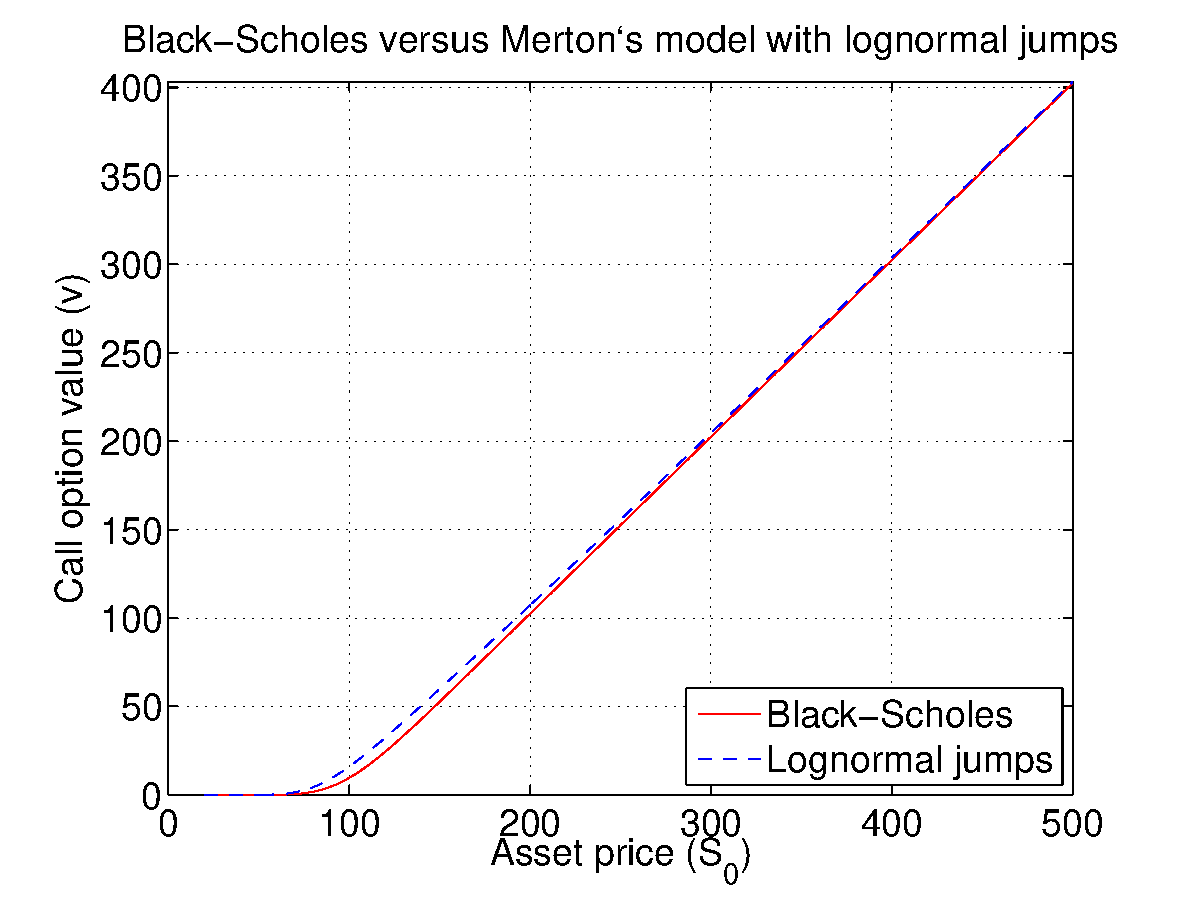
\includegraphics[width=0.6\linewidth]{figures/optionComp.eps}\hspace*{3pt}}
		\subfigure[Difference between \eqref{eqn:mertonSoln} and \eqref{eqn:EUcall}. \label{fig:optionDiff}]{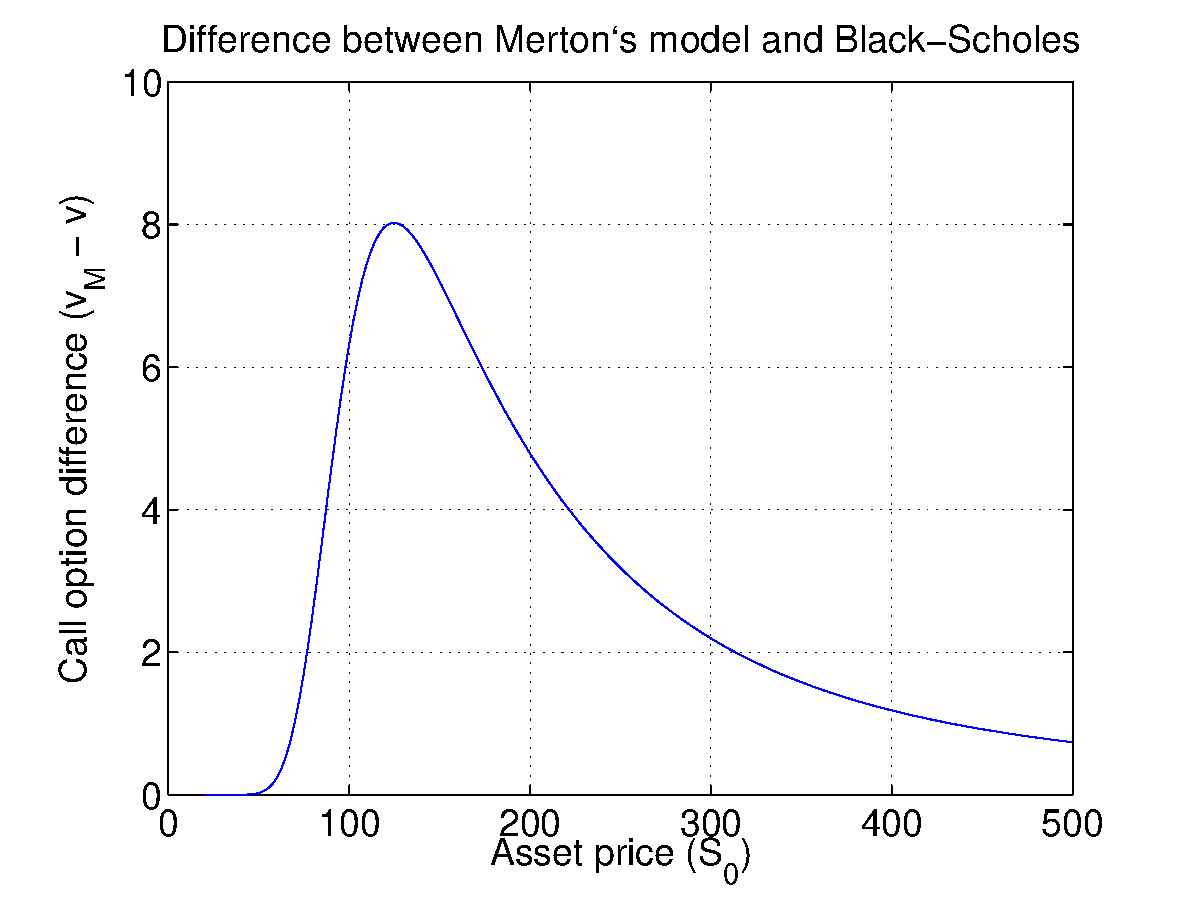
\includegraphics[width=0.6\linewidth]{figures/optionDiff.eps}
			}
		\caption{Call option profiles using \eqref{eqn:EUcall} and \eqref{eqn:mertonSoln}. The financial parameters are $r = 0.05$, $q=0.00$, $\sigma = 0.3$, $T-t = 0.5$, $K = 100$, and $S_0 \in [50,500]$. The lognormal jump parameters are $\lambda = 0.5$, $\mu_Y = -0.90$, and $\sigma_Y = 0.45$.}
		\label{fig:optionComp}
\end{figure}

\section{Example: double exponentially distributed jumps}
We will also demonstrate how to derive a recursive formula for double exponentially distributed jumps. A pricing formula does exist~\cite{Kou2002, Kou2004} for a double exponential jump-diffusion model, but it is expressed in a way that showing equality to the recursive form \eqref{eqn:Fn} is very difficult. Thus only $F_1$ will be determined since it is all that is required to generate the other terms.

Suppose $Y > 0$ is drawn from a double exponential distribution with parameters $\omega_1 > 0, \, \omega_2 > 0$, and $p, \, q \geq 0$ such that $p + q = 1$. Frontczak~\cite{Frontczak2013} gives the corresponding PDF and expectation as
	\begin{equation*}
		f(y) = p\omega_1y^{-\omega_1-1}\1_{\{y\geq 1\}} + q\omega_2y^{\omega_2-1}\1_{\{0 < y < 1\}}, \quad \E[Y^{-\xi}] = \fr{p\omega_1}{\omega_1+\xi} + \fr{q\omega_2}{\omega_2-\xi},
	\end{equation*}
where $\1_{I}$ is the indicator function of the interval $I$. Using \eqref{eqn:Fn}, we get
	\begin{align}
		\label{eqn:doubleExp}
		\begin{split}
		F_1(x) &= \fr{1}{x}\left( p\omega_1\left(\fr{1}{x} \right)^{-\omega_1-1}\1_{\left\{ 1/x \geq 1 \right\}} + q\omega_2\left( \fr{1}{x} \right)^{\omega_2-1}\1_{\left\{ 0 < 1/x < 1 \right\}} \right) \\
		&= p\omega_1x^{\omega_1}\1_{\{ x \leq 1 \}} + q\omega_2x^{-\omega_2}\1_{\{x > 1\}},
		\end{split}
	\end{align}
and from here we can obtain $F_n$ recursively from \eqref{eqn:Fn}. Using this, we can substitute into \eqref{eqn:jumpGeneral} and then \eqref{eqn:optionJump} to find the option price.


\section{Example: gamma distributed jumps}
Whilst a pricing formula for lognormal jumps and double exponential jumps have been derived previously, none exists for gamma distributed jumps. We will show a recursive solution that is still exact and analytic.

Suppose $Y \sim \text{Gamma}(\alpha_Y,\beta_Y)$, where $\alpha_Y > 0$ affects the distribution shape and $\beta_Y > 0$ determines the scale (i.e., how far spread out the distribution is). The associated PDF of $Y$ is given by~\cite{Frontczak2013}
	\begin{equation*}
		f(y) = \fr{1}{\Gamma(\alpha_Y)\beta_Y^{\alpha_Y}}y^{\alpha_Y-1}e^{-y/\beta_Y}, \qquad \E[Y^{-\xi}] = \fr{\beta_Y^{-\xi}\Gamma(\alpha_Y-\xi)}{\Gamma(\alpha_Y)}.
	\end{equation*}
Then using \eqref{eqn:jumpGeneral}, we have
	\begin{equation}
		\label{eqn:gammaJump}
		F_1(x) = \fr{1}{x}\fr{1}{\Gamma(\alpha_Y)\beta_Y^{\alpha_Y}}\left(\fr{1}{x}\right)^{\alpha_Y-1}e^{-1/(x\beta_Y)} = \fr{(x\beta_Y)^{-\alpha_Y}}{\Gamma(\alpha_Y)}e^{-1/(x\beta_Y)},
	\end{equation}
which can then be employed recursively to compute $F_n$. Similarly, $F_n$ can be substituted into \eqref{eqn:jumpGeneral} and then \eqref{eqn:optionJump} to find the corresponding option price.

%We will present two methods to derive the formula: 1) brute-force Mellin inversion but still bypassing direct complex integral computation, and 2) using \eqref{eqn:jumpGeneral} to determine the jump.

%\subsubsection{Brute-force Mellin inversion}
%In order to obtain an analytic pricing formula, we require $\J$. The key to determining $\J$ is to compute $\M^{-1}\left\{ \E[Y^{-\xi}]^n \right\}$. First, we have
%	\begin{equation*}
%		 \E[Y^{-\xi}]^n = \left( \fr{\beta^{-n\xi}}{\Gamma(\alpha)^n} \right)\Gamma(\alpha-\xi)^n.
%	\end{equation*}
%To calculate its inverse Mellin, we require the following lemmas:

%\begin{lemma}
%	\label{lem:2}
%	For some $\beta$, $n \in \mathbb{R}$, we have
%		\begin{equation*}
%			\M\left\{ \fr{\delta\left( x - \fr{1}{\beta^n} \right)}{\beta^n} \right\} = \beta^{-n\xi},
%		\end{equation*}
%	where $\delta$ is the standard Dirac delta function.
%\end{lemma}
%\begin{proof}
%	See Appendix \ref{subsec:lem2}.
%\end{proof}
%\begin{lemma}
%	\label{lem:3}
%	For some $\alpha \in \mathbb{R}$, we have
%		\begin{equation*}
%			\M\left\{ x^{-\alpha}e^{-1/x} \right\} = \Gamma(\alpha - \xi),
%		\end{equation*}
%	where $\Gamma$ is the standard gamma function.
%\end{lemma}
%\begin{proof}
%	See Appendix \ref{subsec:lem3}.
%\end{proof}
%Next, we let $G_n$ be a function such that $\M\left\{ G_n(x) \right\} = \Gamma(\alpha - \xi)^n$. We can rewrite this to be
%	\begin{align*}
%		\M\left\{ G_n(x) \right\} = \Gamma(\alpha - \xi)\Gamma(\alpha - \xi)^{n-1} = \M\left\{ G_1(x) \right\} \M\left\{ G_{n-1}(x) \right\},
%	\end{align*}
%and using the convolution property, we invert this to give
%	\begin{equation*}
%		G_n(x) = \int_0^\infty \fr{1}{z}G_1(z)G_{n-1}\left(\fr{x}{z}\right) \, \d z.
%	\end{equation*}
%Once again, we require a base case to make this recursive formula work. Computing $G_1$ is simple by applying lemma \ref{lem:3} to produce
%	\begin{align*}
%		G_1(x) = \M^{-1}\left\{ \Gamma(\alpha - \xi) \right\} = x^{-\alpha}e^{-1/x}.
%	\end{align*}


\section{Discussion and conclusion}
The key result presented in this chapter was the alternative pricing formula \eqref{eqn:optionJump} for options in a jump-diffusion model for the underlying asset. There are several advantages to this new formula. Firstly, \eqref{eqn:optionJump} is applicable to any general payoff and type of jump. Merton's formula is only applicable when the jump is drawn from a particular distribution, namely, the lognormal distribution. On the other hand, Frontczak's formula is also applicable to any general payoff and type of jump as in \eqref{eqn:optionJump}, but a complex integral has to be evaluated in Frontczak's result and reduces to \eqref{eqn:mertonSoln} for a given payoff and jump. However, the integrals in \eqref{eqn:optionJump} are all real since the Mellin transform inversion has been performed in a different manner to~\cite{Frontczak2013} where the inversion was completed via a complex integral.

Equation \eqref{eqn:optionJump} conveniently represents the standard European option value with shifted parameters and a function which mimics the discontinuous jumps. If multiple types of options are to be priced or if the jump dynamics were changed, \eqref{eqn:optionJump} is in a form whereby any alterations can be easily incorporated since the jump function is completely separated from any other component of the pricing formula. Additionally, the general pricing formula in \cite{Frontczak2013} is expressed as a complex integral with the jump dynamics embedded across multiple terms. In practice, this would be unfavourable as computing complex integrals is relatively expensive when compared to real integrals. %Furthermore, modifying any characteristics regarding the jump (e.g., the distribution) or the payoff would also be quite disadvantageous as it is unclear what terms would need to be amended.
%To complete the result, we also derived a general formula \eqref{eqn:jumpGeneral} which can be computed for any jump following any given distribution. One of the primary advantages of this scheme is the avoidance of complex integration and no ansatz approach is required. Sources like \cite{Frontczak2013} and \cite{Merton1976} often bulk the behaviour of the jump with other terms of financial significance. Whilst it may be economic in terms of notation, it often masks the process that is occurring in regards to the jump-diffusion dynamics within the asset and how that ultimately affects the option pricing process.

Examples were given for the cases where the jumps have distributions that are lognormal, double exponential, and gamma. For lognormal jumps, both \cite{Merton1976} and \cite{Frontczak2013} also derived similar results; Merton's classical formula~\eqref{eqn:mertonSoln} exploited the properties of expectations whilst Frontczak's formula computed the Mellin inverse via algebraic manipulation and the Mellin convolution. Equation~\eqref{eqn:optionLN} was derived using convolution and direct inversion that bypasses the complex integral evaluation employed by Frontczak. One approach used \eqref{eqn:jumpGeneral} to compute the terms recursively whilst the other relied on the properties of the exponential function which simplified the algebra tremendously. It should be emphasized that in \eqref{eqn:optionLN}, having the jump term isolated from the remainder of the formula is convenient since it allows for the pricing process to be modular. That is, one can calculate the necessary jump term before determining the option price at the specified parameter values. Not only is the separation preferable for computation, it reiterates the notion of interchangeability: if the jump dynamics were to change, \eqref{eqn:optionJump} together with \eqref{eqn:jumpGeneral} would be able to accommodate this efficiently. %Albeit complex inversion would produce the exact answer without the potential for a recursive formulation, finding this might be difficult.
Although \eqref{eqn:jumpGeneral} is recursive in the general case, one may obtain some insight into what $F_n$ is by carefully analysing the distribution of the jump. This could ultimately lead to easier calculations. Consequently, it is possible to derive pricing formulas for any types of jumps as shown with the double exponential distribution in \eqref{eqn:doubleExp} and the gamma distribution in \eqref{eqn:gammaJump}. The key is being able to calculate each term in the sequence $F_1, F_2, \ldots$. If the integrals associated with $F_n$ are too complicated to solve analytically, one may resort to numerics to yield approximate solutions to \eqref{eqn:jumpGeneral}. For the double exponential and gamma distributions, we kept the jump terms in a recursive form to demonstrate the capability of \eqref{eqn:jumpGeneral}. However, it is not clear how to obtain a non-recursive form for $F_n$ for double exponentially and gamma distributed jumps as we did for the lognormal jumps.

There is also interest in finding an exact solution for Kou's double exponentially distributed jumps \cite{Kou2002, Kou2004} using \eqref{eqn:optionJump} and \eqref{eqn:jumpGeneral} since recent empirical studies suggest a better model for the asset process involves the jumps following a double exponential distribution. In particular, it may be of interest to see whether or not a Mellin transform route would generate a more elegant and simple solution in lieu of Kou's original solution, which involves the computation of quite complicated $Hh$ functions (see \cite[pp. 691]{Abramowitz1972}). There is also the possibility to extend \eqref{eqn:optionJump} to price American options in jump-diffusion models; this is current work in progress.
	
In conclusion, we have devised and introduced a new scheme for option pricing when the asset follows jump-diffusion dynamics. In particular, we were able to formulate this new model to fit any type of jump. The consequent result can be computed recursively within an infinite sum. This was achieved by implementing the properties of the Mellin transform and the Black-Scholes kernel. We also highlighted how the recursion is handled when the jump is extracted from a lognormal distribution and also provided some insight into how the recursion can be computed when the jump is double exponentially and gamma distributed. 

